\chapter{親子の身長の研究}
% https://twitter.com/ynakahashi1003/status/1610952694767968257

% https://twitter.com/ynakahashi1003/status/1610951312560238594
%参照元の記事、モデルと推定法が区別できてないように感じるし、「線形回帰モデルは実際にこの方法で回帰係数を推定しています」という記述もどんなソフトウェアのどんな関数なのかも書いてなくて正直微妙だなぁ、と。例えばRのlmがあれを計算してるかって言ったらしてないでしょ
\begin{comment}
https://twitter.com/Yh_Taguchi/status/1589082783577944064

https://mathlog.info/articles/2936
https://jp.quora.com/%E7%9B%B8%E9%96%A2%E4%BF%82%E6%95%B0%E3%81%8C0-8%E3%81%A8%E3%82%8F%E3%81%8B%E3%81%A3%E3%81%A6%E3%81%84%E3%82%8B%E9%96%A2%E4%BF%82%E3%82%92%E4%BD%BF%E3%81%A3%E3%81%A6%E7%9B%B8%E9%96%A2%E4%BF%82%E6%95%B01%E3%81%A8/answers/325575293
https://www.jstage.jst.go.jp/article/jve/25/1/25_51/_pdf/-char/ja
https://journals.biologists.com/jeb/article/125/1/29/5000/Fracture-Toughness-Design-In-Horse-Hoof-Keratin?searchresult=1#11919084
https://journals.biologists.com/jeb/article/199/6/1295/7289/The-Effects-of-Salinity-Change-on-the-Exercise?searchresult=1#12304883
https://journals.biologists.com/jeb/article/191/1/19/6760/Variations-in-Force-Time-Histories-of-cat?searchresult=1#13965593
https://www.jstage.jst.go.jp/article/jve/24/1/24_29/_pdf/-char/ja 
\end{comment}

そして、データを使い、よさそうなモデルを探索する。
\section{モデル}
二つの要素に対する3つのモデルを取り上げる。まず、これらの性質について整理する。
\subsection{独立ではない変数を持つモデル}
\begin{enumerate}
 \item $x,y$を確率変数とする。
 \item 平均を$\mu_x,\mu_y$分散を$\sigma^2_x,\sigma^2_y$とする。
\end{enumerate}
このモデルでは、次の$X$と$Y$の共分散という量が定義できる。
\begin{equation*}
 \sigma_{xy} = E[(x-\mu_x)(y-\mu_y)]
\end{equation*}
また、相関係数を次のように定義する。
\begin{equation*}
 \rho_{xy} = \frac{\sigma_{xy}}{\sigma_x\sigma_y}
\end{equation*}




\subsection{正規非独立モデル}



\section{親子の身長の関係}


PearsonとLeeらによる親と子供の身長に関するデータを利用した\footnote{\url{https://vincentarelbundock.github.io/Rdatasets/datasets.html}}。
\begin{table}[http]
 \centering
 %父と息子の統計量を要約したもの
 \begin{tabular}{lrr}
  {} &  child &  parent \\
  count & 179.00 &  179.00 \\
  mean  &  68.33 &   67.08 \\
  std   &   4.53 &    4.03 \\
  min   &  59.50 &   58.50 \\
  25\%   &  64.50 &   64.00 \\
  50\%   &  68.50 &   67.50 \\
  75\%   &  71.50 &   70.50 \\
  max   &  78.50 &   74.50 \\
 \end{tabular}
\end{table}


\begin{table}[http]
 \centering
\begin{tabular}{lrr}
{} &    $\hat{a}$ &      $\hat{b}$ \\
$E_1$ & 0.59 &  29.02 \\
 $E_2$ & 2.16 & -76.69 \\
$E_3$ & 1.25 & -15.76 \\
$E_4$ & 1.13 &  -7.18 \\
\end{tabular}
\end{table}




\if 0
\section{Model I}

ここで、誤差項が確率変数であることを仮定してモデルModel Iを構築する。
\begin{enumerate}
 \item $x_i$は、与えられた定数
 \item $a,b$を実数の定数
 \item $u_i = y_i-a x_i -b$
 \item $u_i \sim N(0,\sigma^2)$
 %\item $E[u_i]=0$。平均は$0$。
 %\item $E[u_j u_i]=0$。無相関。
 %\item $Var[u_i]=0$。分散が均一。
\end{enumerate}
この仮定により構築されるモデルを$M_{I}(a,b; x)$または$M_I(a,b)$と表記する\footnote{正規性の仮定の代わりに、無相関、等しい分散、平均が$0$の仮定を与えるのが簡単な定義である。ここでは、正規性を仮定しておいた}。

\subsection{最尤モデル}
このモデルの最尤モデル$M_{I}^{ML}(\hat{a},\hat{b})$を推定する。
このモデルの尤度は、次式である。
\begin{equation*}
 L = \prod_{i=1}^{n} \frac{1}{\sqrt{2\pi\sigma^2}}\exp\left(-\frac{u_i^2}{2\sigma^2} \right)
\end{equation*}
対数尤度は、以下の式である。
\begin{equation*}
 \log L = -\frac{n}{2}\log 2\pi\sigma^2-\frac{1}{2\sigma^2} \sum_{i=1}^n u_i^2
\end{equation*}
対数尤度の第$1$項は、変数$a,b$が含まれていないので、無視できる。
第二項は、定数の$\frac{1}{2\sigma^2}$部分以外が変数$a,b$に関係している。
以上から、$\log L =0$となる点は、$a,b$に関する偏微分には、


\begin{comment}
これはちがう
 with pm.Model() as model1:  # model specifications in PyMC are wrapped in a with-statement
    # Define priors
    xdata = pm.ConstantData("x", x, dims="obs_id")

    sigma = pm.HalfCauchy("sigma", beta=20)
    #sigma = pm.Uniform("sigma",lower=10**-3,upper=10**3)

    intercept = pm.Normal("intercept", 0, sigma=100)
    #intercept = pm.Beta("intercept",alpha=5,beta=1)
    slope = pm.Normal("slope", 0, sigma=100)
    #intercept = pm.Uniform("intercept",lower=10**-3,upper=10**3)

    #slope = pm.Uniform("slope",lower=10**-3,upper=10**3)

    # Define likelihood
    #likelihood = pm.Normal("y", mu=intercept + slope * xdata, sigma=np.sqrt(slope)*sigma, observed=y)
    #likelihood = pm.Normal("y", mu=intercept + slope * xdata, sigma=sigma/np.sqrt(1+slope**2), observed=y)
    likelihood = pm.Normal("y", mu=(intercept + slope * xdata), sigma=sigma, observed=y)
    # Inference!
    # draw 3000 posterior samples using NUTS sampling
    idata = pm.sample(3000,cores=3)
\end{comment}
\fi

\if 0
\section{Model I'}
実数のペア$(x_1,y_1),(x_2,y_2),\cdots,(x_n,y_n)$が次の線形な関係を持つとする。
\begin{comment}
\begin{equation*}
 u_i =x_i -\frac{y_i-a}{b} \ \ (i=1,2,\cdots,n)
\end{equation*} 
\end{comment}
ここで、誤差項が確率変数であることを仮定してモデルModel I'を構築する。
\begin{enumerate}
 \item $x_i$は、与えられた定数
 \item $a,b$を実数の定数
 \item $u_i = x_i -\frac{y_i-b}{a}$
 \item $u_i \sim N(0,\sigma^2)$
 %\item $E[u_i]=0$。平均は$0$。
 %\item $E[u_j u_i]=0$。無相関。
 %\item $Var[u_i]=0$。分散が均一。
\end{enumerate}
この仮定により構築されるモデルを$M_{I'}(a,b; x)$または$M_{I'}(a,b)$と表記する

\subsection{尤度}
このモデルの対数尤度のうち、
\fi
\begin{comment}
 with pm.Model() as model1:  # model specifications in PyMC are wrapped in a with-statement
    # Define priors
    ydata = pm.ConstantData("y", y, dims="obs_id")

    sigma = pm.HalfCauchy("sigma", beta=10)
    #sigma = pm.Uniform("sigma",lower=10**-3,upper=10**3)

    intercept = pm.Normal("intercept", 0, sigma=100)
    #intercept = pm.Beta("intercept",alpha=5,beta=1)
    slope = pm.Normal("slope", 0, sigma=100)
    #intercept = pm.Uniform("intercept",lower=10**-3,upper=10**3)

    #slope = pm.Uniform("slope",lower=10**-3,upper=10**3)

    # Define likelihood
    likelihood = pm.Normal("x", mu=(ydata-intercept)/slope, sigma=sigma, observed=x)

    # Inference!
    idata = pm.sample(3000,cores=3)
\end{comment}

\if 0
\section{Model II'}

\begin{enumerate}
 \item $x_i-u_i \sim N(0,\sigma^2)$
 \item $y_i-v_i \sim N(0,\sigma^2)$
 \item $a,b$を実数の定数
 \item $v_i -a u_i -b = 0$
\end{enumerate}
この仮定により構築されるモデルを$M_{II'}(a,b; x)$または$M_{II'}(a,b)$と表記する

\subsection{最尤モデル}
このモデルの尤度を計算する。
\begin{eqnarray*}
 L &=& \prod_{i=1}^{n}\frac{1}{\sqrt{2\pi\sigma^2}}\exp\left(-\frac{(x_i-u_i)^2}{2\sigma^2} \right)\prod_{i=1}^{n}\frac{1}{\sqrt{2\pi\sigma^2}}\exp\left(-\frac{(y_i-v_i)^2}{2\sigma^2} \right)\\
 &=& \prod_{i=1}^{n}\frac{1}{\sqrt{2\pi\sigma^2}}\exp\left(-\frac{(x_i-u_i)^2+(y_i-v_i)^2}{2\sigma^2} \right)
\end{eqnarray*}
対数尤度で、

\subsection{モデルの拡張}
このモデルは、次の様に、誤差の分散について拡張できる。
\begin{enumerate}
 \item $x_i-u_i \sim N(0,\sigma_x^2)$
 \item $y_i-v_i \sim N(0,\sigma_y^2)$
 \item $a,b$を実数の定数
 \item $v_i -a u_i -b = 0$
\end{enumerate}
このモデルの最尤推定量は、上記と同様のはずなので、詳しくは計算を行わない。
\begin{eqnarray*}
 \hat{a} &=& \frac{Q_{yy}-\lambda Q_{xx}+\sqrt{(Q_{yy}-\lambda Q_{xx})^2+4\lambda Q_{xy}}}{2Q_{xy}} \\
 \hat{b} &=& \bar{y}-\hat{a}\bar{x}
\end{eqnarray*}
ここで、$\lambda = \frac{\sigma_x^2}{\sigma_y^2}$である。

\section{Model II}

ここで、誤差項が確率変数であることを仮定してモデルModel Iを構築する。
\begin{enumerate}
 %\item $x_i$は、与えられた定数
 \item $a,b$を実数の定数
 \item $u_i = y_i-a x_i -b$
 \item $u_i \sim N(0,a\sigma^2)$
 %\item $E[u_i]=0$。平均は$0$。
 %\item $E[u_j u_i]=0$。無相関。
 %\item $Var[u_i]=0$。分散が均一。
\end{enumerate}
この仮定により構築されるモデルを$M_{II}(a,b; x)$または$M_{II}(a,b)$と表記する。
\subsection{最尤モデル}
\begin{equation*}
 L = \prod_{i=1}^n\frac{1}{\sqrt{2\pi\sigma^2}}\exp\left(-\frac{(\frac{u_i}{\sqrt{a}})^2}{2\sigma^2} \right)
\end{equation*}
この尤度で、最大化される部分は次の式で表される。
\fi




\begin{comment}
 \begin{table}
 \begin{tabular}{llll}
  名前 & 最小化要素 & 最小化関数 & \\
  \hline \hline\\
  Model I regression & && \\

  Regression &$y$軸方向の変動を最小化 & $s_{y,x}(\Delta y^2)$ & \\
  Model II regression & && \\

  標準主軸回帰 &  $x,y$軸方向から直線への変動を最小化 & $\Delta x\Delta y$ &  \\
  standard major axis(SMA回帰) &&& \\
  major axis regression, &&& \\
  幾何平均回帰, Reduced major axis(RMA) &&& \\
  主成分分析(Principal component analysis) &観測点$(x,y)$から直線への最短距離を最小化 & $s\Delta h^2$ & \\

  %Deming回帰 &  & $s_d$ & \\
 \end{tabular}
\end{table}

幾何平均回帰は,標準化主軸回帰(Standardised major axis(SMA回帰))標準主軸 (Standard major axis)回帰,縮小長軸(Reduced major axis, RMA)回帰
Principal component analysis 主成分回帰は,主軸回帰,最大軸回帰 MA(Major axis), Orthogonal regression


\begin{table}
 \begin{tabular}{llll}
  名前 & 最小化要素 & 最小化関数 & \\
  \hline \hline
  Model I regression & && \\

  Regression &$y$軸方向の変動を最小化 & $s_{y,x}(\Delta y^2)$ & \\
  Model II regression & && \\

  SMA回帰 &  $x,y$軸方向から直線への変動を最小化 & $\Delta x\Delta y$ &  \\
  PCA &観測点$(x,y)$から直線への最短距離を最小化 & $s\Delta h^2$ & \\

  %Deming回帰 &  & $s_d$ & \\
 \end{tabular}
\end{table}

\end{comment}




\section{観測点を直線により予測する}
実数のペア$(x_1,y_1),(x_2,y_2),\cdots,(x_n,y_n)$が次の線形な関係を持つとする。
\begin{equation*}
 y_i = ax_i+b+u_i, \ \ (i=1,2,\cdots,n)
\end{equation*}

点A$(x,y)$と直線の関係を図\ref{fig:RegressionModel}に示しす。
点$A$と同じ$x$座標の直線上の点$D$は、$(x,ax+b)$である。
点$A$と同じ$y$座標の直線上の点$B$は、$(\frac{y-b}{a},y)$である。
$DA$間の距離を$|\Delta y$、$BA$間の距離を$|\Delta x|$で表す。
$BA$間の距離は、$|\Delta x| = \frac{|\Delta y|}{a}$である。
これは、
\begin{eqnarray*}
 \Delta x &=& x-\frac{y-b}{a} \\
 &=& \frac{ax+b-y}{a} \\
 &=& \frac{\Delta y}{a}
\end{eqnarray*}
より明らかである。
また、点$A$から直線に向けて垂直に下した点を$C$とする。
$AC$間の距離は、$\frac{|y-ax-b|}{\sqrt{a^2+1}}$である。
また、三角形$ABD$の面積の倍は$\Delta x\Delta y =\frac{\Delta x^2}{a}$である。


\begin{figure}
 \begin{center}
  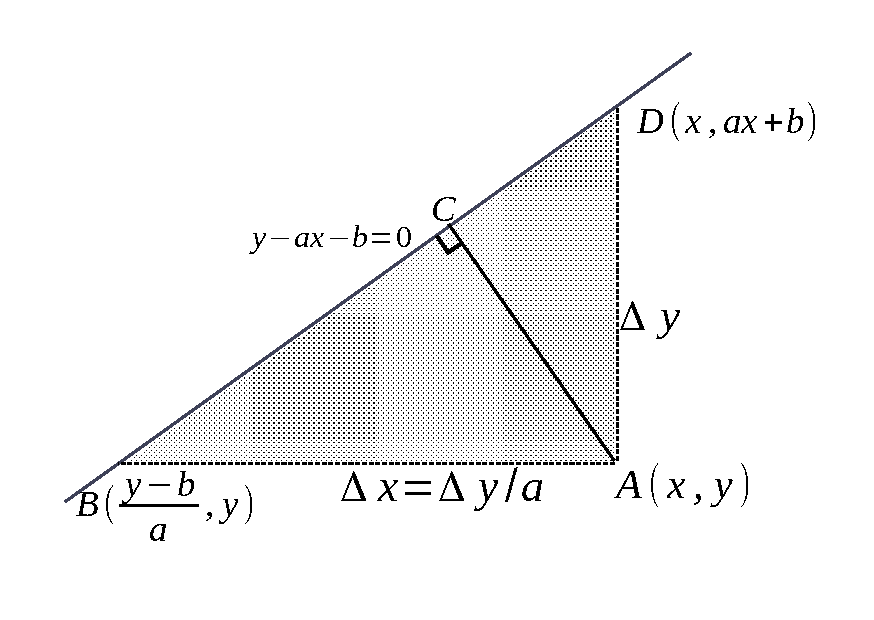
\includegraphics[width=8cm]{./image/16_/RegressionModel.pdf}
  \caption{点$A$と直線$Y=aX+b$の関係}
  \label{fig:RegressionModel}
 \end{center}
\end{figure}

以上から点と直線の距離について4つの方法で定義ができることがわかる。
また、各点についてそれぞれの式を和にすると、以下の通りである。
\begin{enumerate}
 \item 点と直線の最短距離$AC$:$E_3 = \sum (\frac{\Delta y_i}{\sqrt{1+a^2}})^2$
 \item $y$軸に関する距離$AD$:$E_1=\sum \Delta y_i^2$
 \item $x$軸に関する距離$AB$:$E_2=\sum  (\frac{\Delta y_i}{a})^2=\sum (\Delta x)^2$
 \item 面積を元にした距離$AB\times AD$:$2\times E_4 = \sum (\frac{\Delta y_i}{\sqrt{a}})^2$
\end{enumerate}

ある点と直線への距離が離れていれば、その点への予測ができていないことを示し、近ければ、それなりによい予測をしているだろう。
このことから、$E_j$が小ければ、それぞれの距離の意味で、各々の点と直線が近いはずである。
そこで、まず$E_j$が最も小さくなるように直線のパラメータ$(a_j,b_j)(j=1,2,3,4)$を定める。
さらに、それぞれの直線の性質についてしらべる。


\paragraph{点と直線の最短距離}
点と直線の距離について証明を行う。大抵の高校数学の教科書には記述されているはずである。
点$A(x,y)$から直線$Y-aX-b=0$への直線距離$d$の関係を求める。
点$B$は、点$A$を$x$方向に移動させたとき、直線と交わる点である。つまり点$B$は、$(\frac{y-b}{a},y)$である。
また点$D$は、点$A$を$y$方向に移動させたとき、直線と交わる点である。つまり点$D$は、$(x,ax+b)$である。
点$C$は、点$A$を直線$Y-aX-b=0$へ垂直に下ろした点である。この$AC$間の距離を$d$とする。
直線$DA$と直線$AC$のなす角度を$\theta$とする。
このとき、次の関係が求められる。
\begin{eqnarray*}
 \sin \theta &=& \frac{AC}{BA}\\
 &=& \frac{d}{x-\frac{y-b}{a}}\\
\cos\theta &=& \frac{AC}{DA}\\
&=& \frac{d}{ax+b-y}
\end{eqnarray*}
また、$\cos^2\theta+\sin^2\theta$を計算する。
\begin{eqnarray*}
 \cos^2\theta+\sin^2\theta &=& \frac{d^2}{(y - \frac{y-b}{a})^2}+\frac{d^2}{(ax+b-y)^2}\\
 &=& \frac{d^2(a^2+1)}{(ax+b-y)^2} \\
 &=& 1
\end{eqnarray*}
この式を$d$について解く。
\begin{equation*}
 d^2 = \frac{(y-ax-b)^2}{a^2+1}
\end{equation*}


\begin{figure}
 \begin{center}
  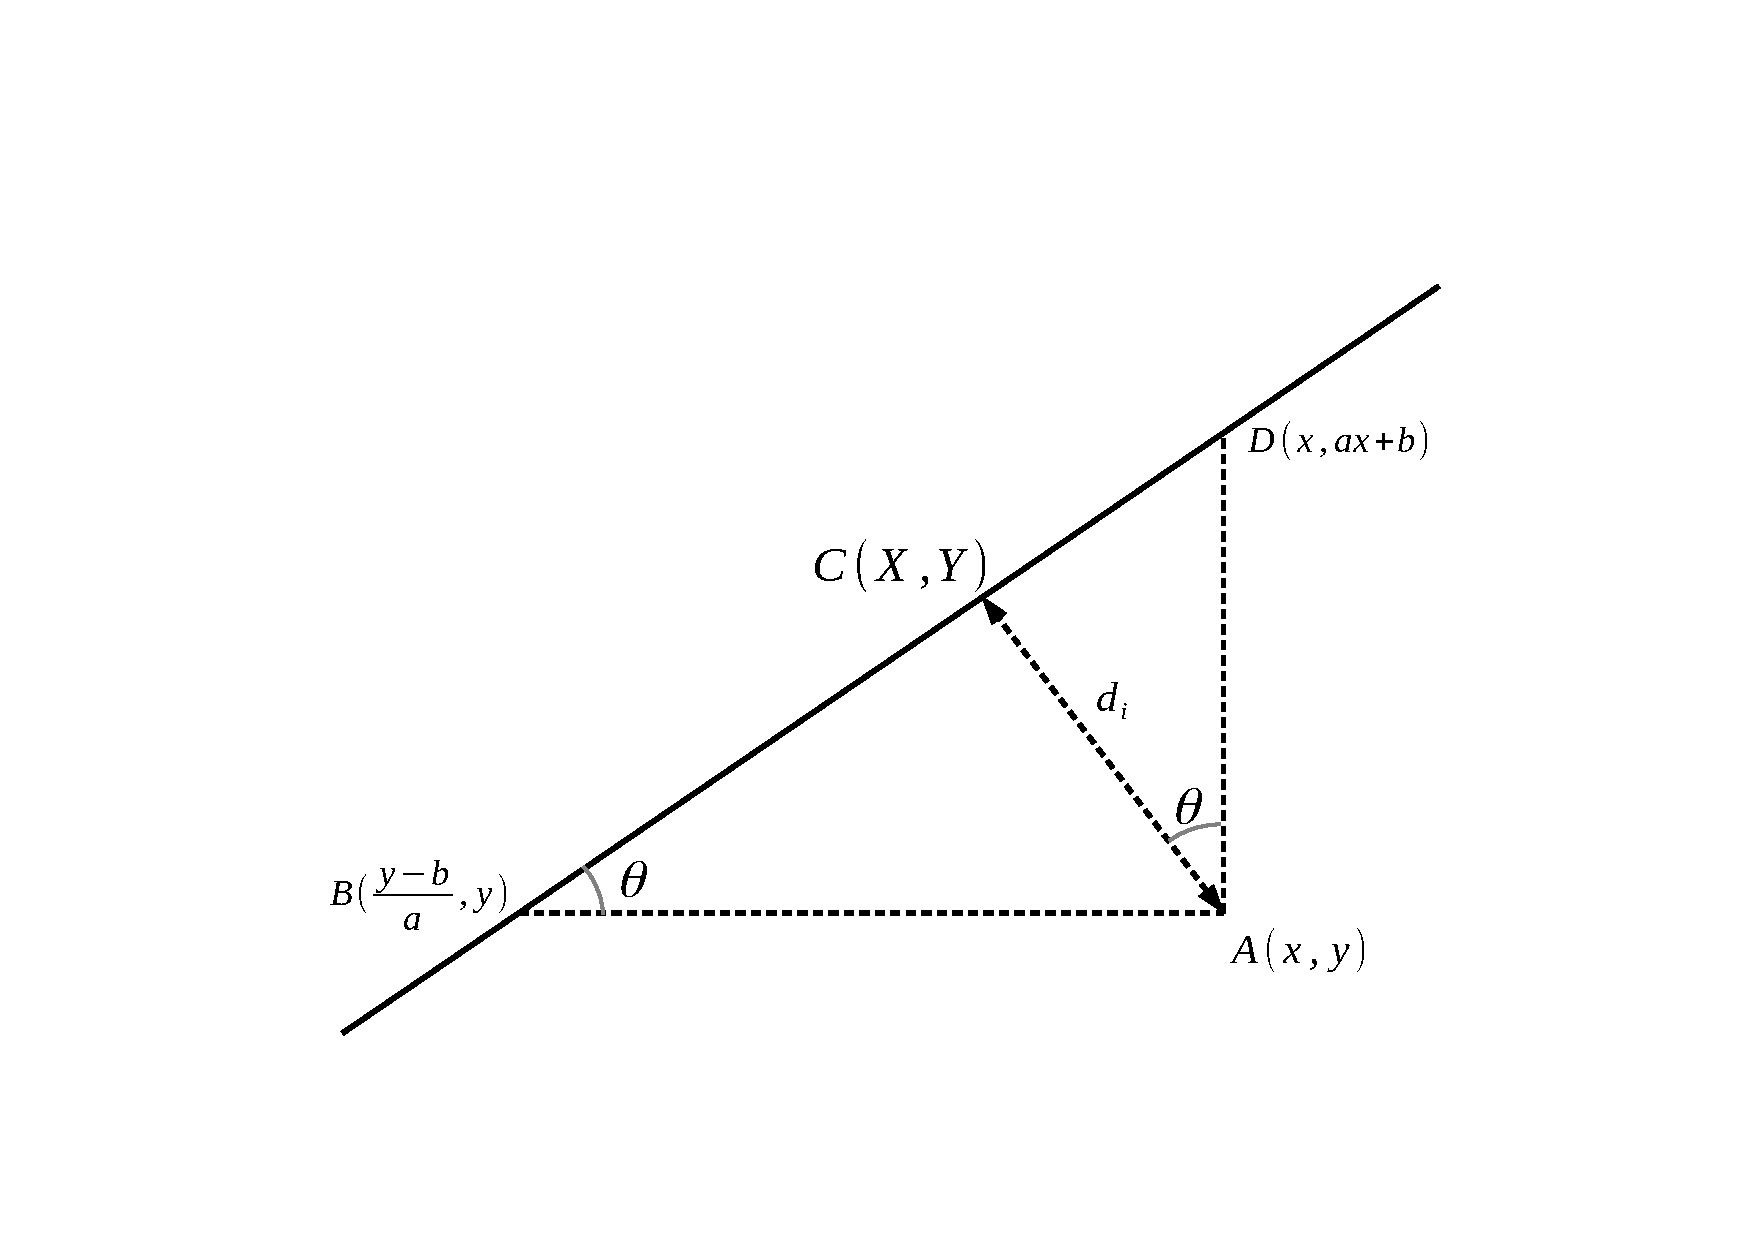
\includegraphics[width=8cm]{./image/16_/point_line_distance.pdf}
  \caption{点$A$から直線$Y=aX+b$への直線距離$d$の関係}
  \label{fig:point_line_distance}
 \end{center}
\end{figure}

\paragraph{$\sum \Delta y_i^2$に関する計算}
\begin{equation}\label{sum_square_error}
 E_1 = \sum_{i=1}^n u_i^2 = \sum_{i=1}^n (y_i-a x_i-b)^2
\end{equation}
式\ref{sum_square_error}にいくらか式変形を行う。
\begin{eqnarray*}
 \sum_{i=1}^n (y_i-a x_i-b)^2 &=& \sum_{i=1}^n \{(y_i-\bar{y}) - a(x_i-\bar{x}) +(\bar{y}-b-a\bar{x})  \}^2\\
 & =& \sum_{i=1}^n \{ (y_i-\bar{y})-a(x_i-\bar{x})  \}^2+n(\bar{y}-b-a\bar{x})^2 \\
 &=& Q_{xx}a^2-2Q_{xy}a+Q_{yy}+n(\bar{y}-b-a\bar{x})^2
\end{eqnarray*}
ここで、以下の式を定義しておく。
\begin{eqnarray*}
 \bar{x} &=& \frac{1}{n}\sum_{i=1}^n x_i \\
 \bar{y}&=& \frac{1}{n}\sum_{i=1}^n y_i \\
 Q_{xx} &=& \sum_{i=1}^n (x_i-\bar{x})^2 \\
 Q_{yy} &=& \sum_{i=1}^n (y_i-\bar{y})^2 \\
 Q_{xy} &=& \sum_{i=1}^n (x_i-\bar{x})(y_i-\bar{y}) \\
\end{eqnarray*}

\paragraph{$E_1$}
まず、式\ref{sum_square_error}を、$b$について偏微分を行う。
\begin{equation*}
 \frac{\partial E_1}{\partial b} = -2(\bar{y}-b-a\bar{x})
\end{equation*}
この式が$0$となる$b$について解くと、次が求まる。
\begin{equation*}
 \hat{b} = \bar{y}-\hat{a}\bar{x}
\end{equation*}

また、$E_1$を$a$について偏微分を行う。
\begin{eqnarray*}
 \frac{\partial E_1}{\partial a} = 2aQ_{xx}-2Q_{xy}
\end{eqnarray*}
以上から、$a$が求められる。
\begin{equation*}
 \hat{a} = \frac{Q_{xy}}{Q_{xx}}
\end{equation*}


\paragraph{$E_2$}
$a,b$に関係する部分は、以下の式である。
\begin{equation*}
 E_2 = \frac{1}{a^2}(Q_{xx}a^2-2Q_{xy}a+Q_{yy}+n(\bar{y}-b-a\bar{x})^2)
\end{equation*}
$E_2$の$b$に関する偏微分が$0$になる点は、以下の式である。
\begin{equation*}
 \hat{b} = \bar{y}-\hat{a}\bar{x}
\end{equation*}
また、$E_2$の$a$に関する偏微分を計算する。
\begin{eqnarray*}
 \frac{\partial E_2}{\partial a} &=& -\frac{2}{a^3}(a^2Q_{xx}-2Q_{xy}a+Q_{yy}) \\
& & +\frac{1}{a^2}(2aQ_{xx}-2Q_{xy})
\end{eqnarray*}
この式を$a$についてとくと、最尤推定量がもとめられる。
\begin{equation*}
 \hat{a}= \frac{Q_{yy}}{Q_{xy}}
\end{equation*}

\paragraph{$E_3$}

変数$a,b$に関連のある項を計算する。
\begin{eqnarray*}
 h(a,b) = \sum_{i=1}^n (x_i-u_i)^2+(y_i-v_i)^2
\end{eqnarray*}
対数尤度を最大化するかつ$v_i -a u_i -b = 0$を満すものを求める。

これは難しいので、幾何学的な考察を行う。
$h(a,b)$は、$(x_i,y_i)$から$(u_i,v_i)$上への距離の和を示している。これを最小化するのは、$(x_i,y_i)$から直線$v_i-a u_i-b=0$への直線距離を最小化しているのに等しい。
このことから、直線から点への距離の公式から、その和は、次の式で表すことができる。
\begin{equation*}
 E_3 = \sum_{i=1}^n \frac{ (y_i-b-ax_i)^2}{1+a^2}
\end{equation*}
$E_1$との違いは、分母に$(1+a^2)$の項が加わったことである。これが、推定量に違いを生じさせる。
式$E_3$を展開していく。
\begin{comment}
\begin{eqnarray*}
 (1+a^2)E_3 &=& \sum_{i=1}^n \{ (y_i-\bar{y})-a(x_i-\bar{x})+(\bar{y}-a\bar{x}-b) \}^2 \\
 &=& \sum_{i=1}^n \{  (y_i-\bar{y})-a(x_i-\bar{x}) \}^2+n(\bar{y}-a\bar{x}-b)^2 \\
 &=& Q_{yy}+a^2 Q_{xx}-2aQ_{xy}+n(\bar{y}-a\bar{x}-b)^2 \\
\end{eqnarray*} 
\end{comment}


\begin{equation*}
 (1+a^2)E_3 = Q_{yy}+a^2 Q_{xx}-2aQ_{xy}+n(\bar{y}-a\bar{x}-b)^2 \\
\end{equation*}
この式を最小化する。まず$b$により偏微分を行う。
\begin{eqnarray*}
 \frac{\partial E_3}{\partial b} = -2n(\bar{y}-a\bar{x}-b)
\end{eqnarray*}
これが$0$になるので、最尤推定した$\hat{b}$は次の式となる。
\begin{equation*}
 \hat{b} = \bar{y}-\hat{a}\bar{x}
\end{equation*}
次に、$a$について偏微分をおこなう\footnote{ $(f/g)'= \frac{f'g-fg'}{g^2}$ }。
\begin{eqnarray*}
\frac{\partial E_3}{\partial a} = \frac{(2aQ_{xx}-2Q_{xy})(1+a^2)-2a(Q_{yy}+a^2Q_{xx}-2aQ_{xy})}{(1+a^2)^2}
\end{eqnarray*}
分子を整理すると、次の式となる。
\begin{equation*}
 Q_{xy}a^2-a(Q_{yy}-Q_{xx})-Q_{xy}
\end{equation*}
$\frac{\partial E_3}{\partial a} =0$より、$a$について解く。
上式は、$a$に関する二次方程式なので、$a$を解く。
\begin{equation*}
 \hat{a} = \frac{Q_{yy}-Q_{xx}+\sqrt{(Q_{yy}-Q_{xx})^2+4Q_{xy}}}{2Q_{xy}}
\end{equation*}




\paragraph{$E_4$}
\begin{eqnarray*}
 E_4=\sum_{i=1}^n u_i^2 &=& \sum_{i=1}^n \frac{1}{a}(y_i-a x_i-b)^2 \\
 &=& \frac{1}{a}(Q_{xx}a^2-2Q_{xy}a+Q_{yy}+n(\bar{y}-b-a\bar{x})^2)
\end{eqnarray*}
ここで、$E_4$の$b$に関する偏微分が$0$となる$b$を求める。
\begin{equation*}
 \hat{b} = \bar{y}-\hat{a}\bar{x}
\end{equation*}
同様に、$E_4$の$a$に関する偏微分が$0$となる$a$を求める。
\begin{eqnarray*}
 \frac{\partial E_4}{\partial b} &=& \frac{1}{a}(2aQ_{xx}-2Q_{xy})\\
&& -\frac{1}{a^2}(Q_{xx}a^2-2Q_{xy}a+Q_{yy}) = 0 \\
\rightarrow && a^2 Q_{xx}-Q_{yy} = 0
\end{eqnarray*}
以上から、最尤推定量が求められる。
\begin{equation*}
 \hat{a}= \sqrt{\frac{Q_{yy}}{Q_{xx}}}
\end{equation*}
この式は、$\frac{Q_{xy}}{Q_{xx}}$と$\frac{Q_{yy}}{Q_{xy}}$の幾何平均と一致する。
ここで、幾何平均は、$0$より大きな数$a_1,a_2,\cdots,a_n$について、次の量のことである。
\begin{equation*}
 (a_1a_2\cdots a_n)^{\frac{1}{n}}
\end{equation*}

\subsection{まとめ}
実際のところ、$E_1$の中にも$a$に係る項が入っているので、$a$がどのような値になるかは推測しにくい。気持ちとして以下のようになることが考えられる。
$E_2,E_3$は、分母に傾き$a$が入っている。この項が$1$より大きければ、$E_2,E_3$を小くし、$1$より小ければ、$E_2,E_3$は大きくなる。
このことから、$E_2,E_4$において$a$は$1$よりも大きくなりがちであることが予想される。
$E_3$については、分母に$1+a^2$の項があるため、任意の$a$において、$E_3$を小くしてくれそうである。

\paragraph{$a_1$と$a_2$の大小関係}
\begin{eqnarray*}
 \frac{1}{a_2}a_1 &=& \frac{Q_{xy}}{Q_{yy}}\frac{Q_{xy}}{Q_{xx}} \\
 &=& \frac{Q^2_{xy}}{Q_{xx}Q_{yy}}
\end{eqnarray*}
ここで、$r^2$を以下のように定める。
\begin{equation*}
 r^2 = \frac{Q^2_{xy}}{Q_{xx}Q_{yy}}
\end{equation*}
この$r^2$は$1$以下であることから、
\begin{equation*}
 a_1 \leq a_2
\end{equation*}
であることがわかる。
これは、$E_2$の直線の傾きは$E_1$の直線の傾きよりも急であることを示唆している。

\paragraph{$r^2\leq 1$の証明}
コーシーシュワルツの不等式
$a_1,a_2,\cdots,a_n,b_1,b2,\cdots,b_n$を実数とする。
\begin{equation*}
 (\sum_{i=1}^n a_i b_i)^2 \leq (\sum_{i=1}^n a_i^2)(\sum_{i=1}^n b_i^2)
\end{equation*}
である。統合成立は、$a_i=0$または$b_i=0$または$b_1/a_1=b_2/a_2=\cdots=b_n/a_n$が成り立つときである。

このことを利用する。$a_i=x_i-\bar{x},b_i=y_i-\bar{y}$とおく。
\begin{equation*}
 \left(\sum_{i=1}^n (x_i-\bar{x})(y_i-\bar{y})\right)^2 \leq  \sum_{i=1}^n(x_i-\bar{x})^2\sum_{i=1}^n(y_i-\bar{y})^2
\end{equation*}
このことから、$r^2\leq 1$がわかる。

\paragraph{$a_1,a_2,a_4$の関係}
相加相乗平均とは次のことである。
実数$a,b>0$について、次が成り立つ。
\begin{equation*}
 \frac{a+b}{2} \geq \sqrt{ab}
\end{equation*}

ここで、$a=a_1,b=a_2$とおくと次がわかる。
\begin{equation*}
 \frac{a_1+a_2}{2}  \geq  \sqrt{a_1 a_2} = a_4
\end{equation*}
このことから、$a_4$は$a_1,a_2$の平均値よりも小さい。



\begin{table}[http]
 \centering
 \begin{tabular}{lcc}
  & a & b\\
  \hline 
  $E_1$ & $\frac{Q_{xy}}{Q_{xx}}$  &$\bar{y}-\hat{a}\bar{x}$ \\
  $E_2=\frac{1}{a^2}E_1$ & $\frac{Q_{yy}}{Q_{xy}}$ & $\bar{y}-\hat{a}\bar{x}$ \\
$E_3=\frac{1}{1+a^2}E_1$ & $\frac{Q_{yy}-Q_{xx}+\sqrt{(Q_{yy}-Q_{xx})^2+4Q_{xy}^2}}{2Q_{xy}}$ & $\bar{y}-\hat{a}\bar{x}$ \\
  $E_4=\frac{1}{a}E_1$ & $\sqrt{\frac{Q_{yy}}{Q_{xx}}}$ & $\bar{y}-\hat{a}\bar{x}$
 \end{tabular}
\end{table}

